

\section{Performance measures}
In aiding the quantification of the two proposed control measures, a Fitts' law test will be used. A general Fitts' law test incorporates five different performance metrics in the evaluation of movement.\cite{Kamavuako2014,Scheme2013} The five metrics and their description can be found in table \ref{fig:Fitts}    

  \begin{figure}[H]                                         
  	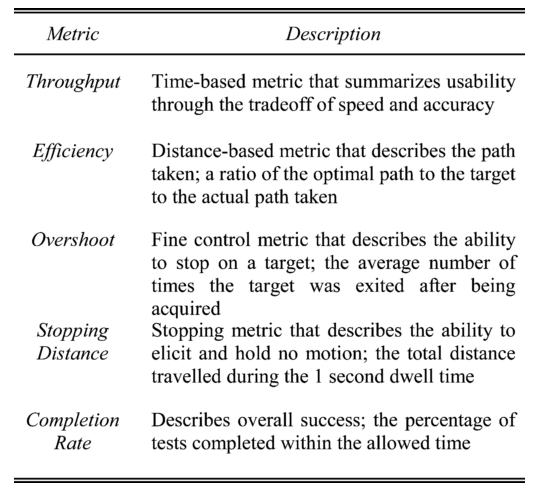
\includegraphics[width=.4\textwidth]{figures/Fitt}  
  	\caption{The table shows the metrics used in a generel Fitts' law test, and a description of these.\cite{Scheme2013}}
  	\label{fig:Fitts} 
  \end{figure} 